\documentclass[11pt,a4paper]{article}
\usepackage[utf8]{inputenc}
\usepackage[T1]{fontenc}
\usepackage{amsthm} %numéroter les questions
% \usepackage[frenchb]{babel}
\usepackage{datetime}
\usepackage{xspace} % typographie IN
\usepackage{hyperref}% hyperliens
\usepackage[all]{hypcap} %lien pointe en haut des figures
\usepackage[french]{varioref} %voir x p© y
\usepackage{fancyhdr}% en têtes
%\input cyracc.def
\usepackage[]{graphicx} %include pictures
\usepackage{pgfplots}
\usepackage[ ]{circuitikz}
\usepackage{ifthen}

\usepackage[top=1.3 in, bottom=1.3 in, left=1.3 in, right=1.3 in]{geometry} % Yeah, that's bad to play with margins
\usepackage[]{pdfpages}

\usepackage[]{attachfile}

\usepackage[many]{tcolorbox}

\newdateformat{mydate}{v2.0.0}%hack pour remplacer \THEYEAR


\newboolean{corrige}
\ifx\correction\undefined
\setboolean{corrige}{false}% pas de corrigé
\else
\setboolean{corrige}{true}%corrigé
\fi

\setboolean{corrige}{false}% pas de corrigé

\newboolean{annexes}
\setboolean{annexes}{true}%annexes
%\setboolean{annexes}{false}% pas de annexes

\definecolor{darkblue}{rgb}{0,0,0.5}

\newboolean{mos}
%\setboolean{mos}{true}%annexes
\setboolean{mos}{false}% pas de annexes

\usepackage{aeguill} %guillemets

%% fancy header & foot
\pagestyle{fancy}
%Numero du TP :
\def \labonumber {Laboratory work 1 }
\lhead{[ELEC-H-310] Digital Choucroute\\ \labonumber}
\rhead{\mydate\today\\ page \thepage}
\chead{\ifthenelse{\boolean{corrige}}{Corrigé}{}}
\cfoot{}
%%

\pdfinfo{
/Author (ULB -- BEAMS)
/Title (\labonumber ELEC-H-310)
/ModDate (D:\pdfdate)
}

\hypersetup{
pdftitle={\labonumber [ELEC-H-310] Digital Choucroute},
pdfauthor={ULB -- BEAMS},
pdfsubject={}
}

\theoremstyle{definition}% questions pas en italique
\newtheorem{Q}{Question}[] % numéroter les questions [section] ou non []

\newcommand{\reponse}[1]{% pour intégrer une réponse : \reponse{texte} : sera inclus si \boolean{corrige}
	\ifthenelse {\boolean{corrige}} {\paragraph{Answer:} \color{darkblue}   #1\color{black}} {}
 }

\newcommand{\addcontentslinenono}[4]{\addtocontents{#1}{\protect\contentsline{#2}{#3}{#4}{}}}

\date{\vspace{-1.7cm}\mydate\today}
\title{\vspace{-2cm} \labonumber\\ Digital Electronics [ELEC-H-310]\\ Introduction to PSOC\ifthenelse{\boolean{corrige}}{\\Solution}{}}

%\author{\vspace{-1cm}}%\textsc{Yannick Allard}}

\setlength{\parskip}{0.2cm plus2mm minus1mm} %espacement entre §
\setlength{\parindent}{0pt}

\begin{document}
\pagestyle{empty}
\maketitle
% \vspace*{-1cm}
\section*{Purpose}
The purpose of this lab is to introduce a commonly used microcontroller family: PSOC from Cypress.
Few simple systems based on input/output (IO) will be realized.
In parallel, you will get familiar with C language.
Afterwards, you will learn how to realize a time-driven program.

% \section*{Prérequis}
% Il est encore conseillé de lire les sections 1 à 5 du complément «Programmation d’une carte à microcontrôleur».

\section*{Objectives}
At the end of this lab, you must be able to:
\begin{itemize}
\item Write simple programs for a microcontroller.
\item Explain the idea of IOs and output current.
\item Use asynchronous elements in your code through timers.
\end{itemize}
\newpage{}


\section{Introduction}
During the six laboratories illustrating the theory, you will use a single-board microcontroller.
Besides the programming, you must understand the functioning of the various peripherals and interface them with the external world.

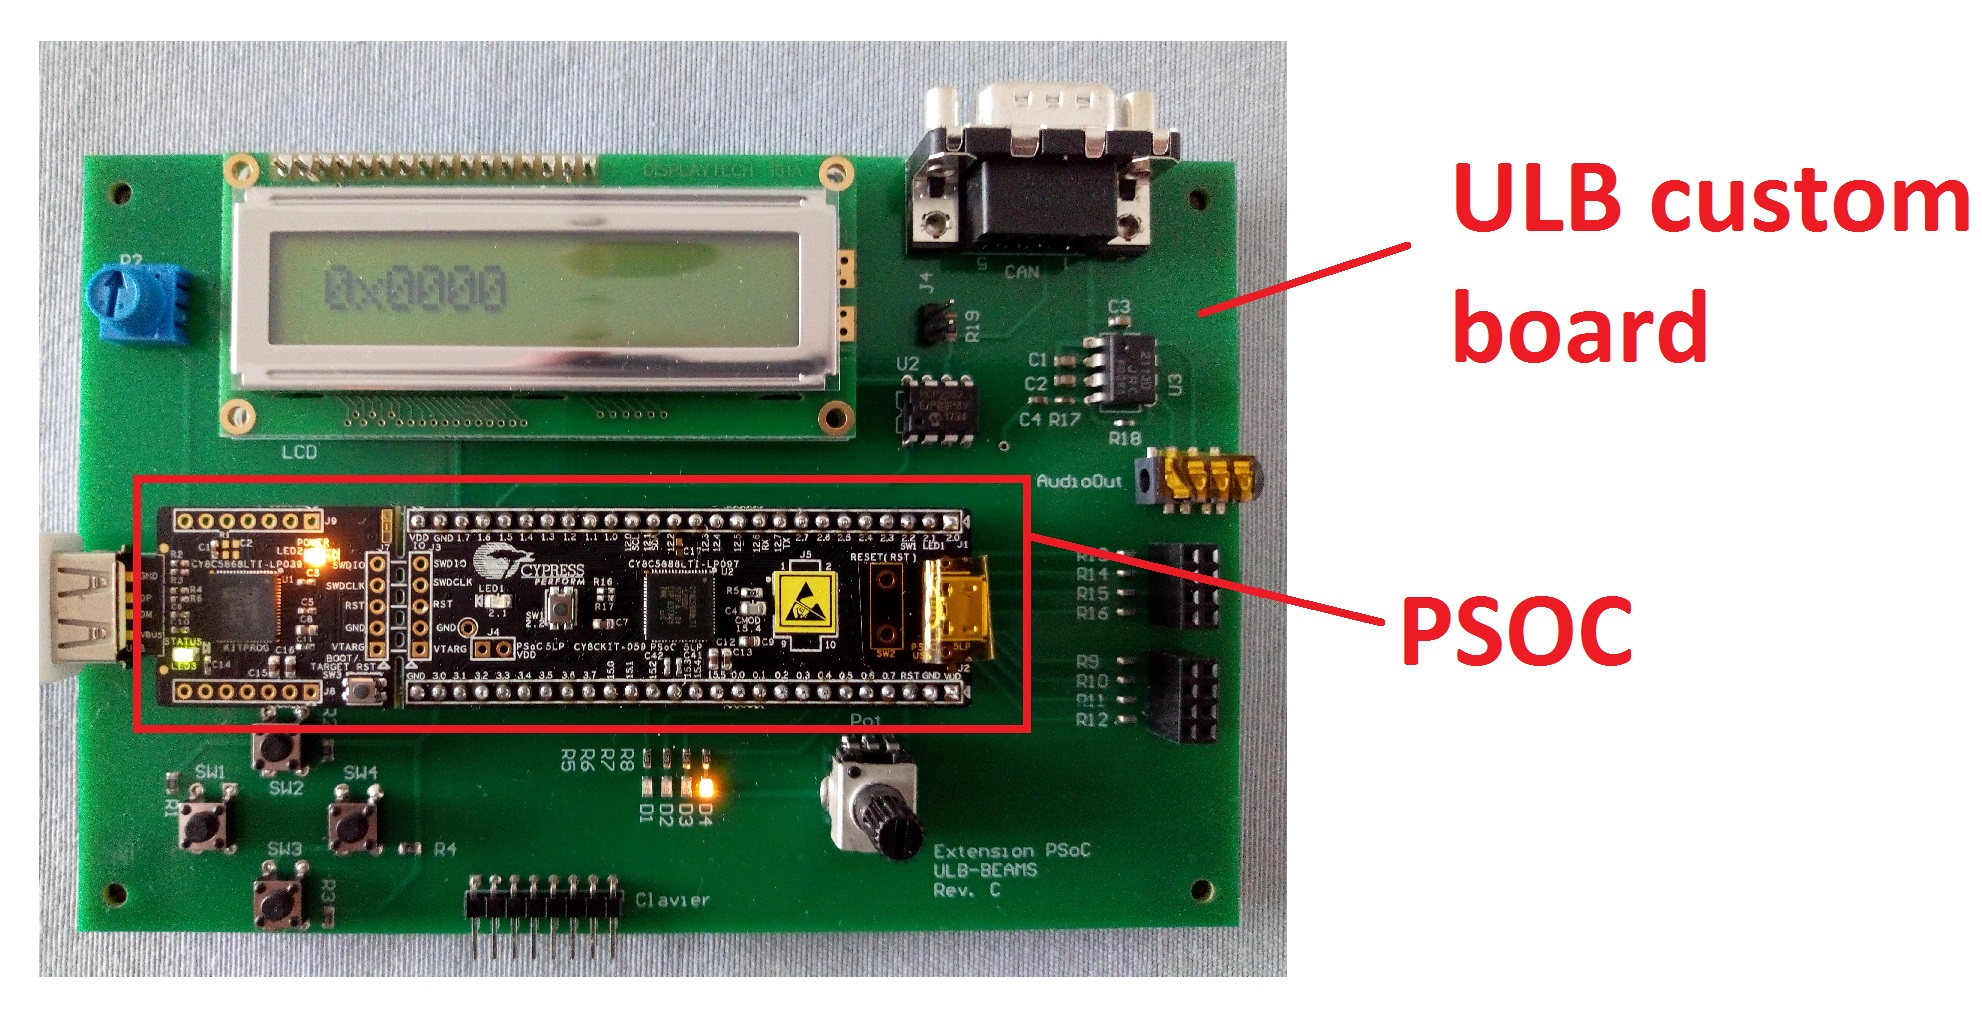
\includegraphics[width=\textwidth]{ULB_custom_board_and_PSOC}

This first lab will help you to get familiar with the board and use some peripherals. You will learn to interact simply with the microcontroller on the board.

The functioning of the PSOC board is extensively documented in the PSOC datasheets and through online courses: \url{www.cypress.com/psoc101}. For the first lab, we advise you to watch the following videos: ``1. Software output pins" and ``2. Software input pins". 

Let us first note that the microcontroller system you will be using during the labs is composed of two boards, as shown in the picture above. The first one is the PSOC microcontroller, which contain the actual microcontroller system. The second one is a ULB-custom-designed extension board, that contains, switches, LEDs, a screen, potentionmeter, etc. The architecture of the extension board and the mapping the to PSOC input/output pins is given in the appendix ``Extension PSOC''. 





\section{Basic programmation: use of inputs and outputs}
Your first program will interface two sorts of IOs: push-buttons and LEDS.
The specifications are simple: the LEDs D1-D4 must switch on when buttons SW1-SW4 are pushed, and switch off when these buttons are released.

\begin{itemize}
	\item Locate the different peripherals present on the extension board and named in the appendix ``Extension PSOC'' (LEDs, push-buttons, potentiometer, analog output connected to power amplifier, etc.). To which outputs of the PSOC 
	\item Identify which PSOC pin number connects to each LED and each switch of the extension board. 
	\item Create a new project in PSOC creator. The device you are using is a ``PSoC 5LP", ``CY8C5888L TI-LP097".
	\item In the topDesign.cysch file, instantiate the LEDs as digital outputs (use the ``Strong Drive'' mode). When double-clicking on a component in the topDesign.cysch file, you open it's customized menu, where you can select options of the component. Similarly to the video tutorial on PSOC 101, you can add the resistors, diode and ground of the extension board as off-chip component for more clarity in your design (use the schematics in the appendix ``Extension PSOC'' for exact component values and mapping). 
	\item In the topDesign.cysch file, instantiate the switches as digital inputs (use the ``High Impedance Digital'' mode). Again, you can add the elements of the extension board as off-chip components in your design for more clarity. 
	\item In the projectName.cydwr file, associate each LED and each switch the appropriate PSOC pin number you identified before. 
	
	\item Now go the file where you write the firmware code (i.e. main.c). You can now write the code fulfilling the specifications: 
	\begin{itemize}
		\item Locate the for(;;) loop.
        This endless loop contains the tasks that must run continuously, while the code placed before and after this loop is only executed once and is mainly used to configure the peripherals and define the variables.
		\item Write how the LEDs and switches should behave. When double-clicking on a component in the topDesign.cysch file, you open it's customized menu. There is a button to rapidly access the datasheet of the component. Use the ``Application Programming Interface'' section to determine how to use the component from the firmware (i.e. the main.c-file). 
		\item Build, compile and load it on the $\mu$C board, then check its behavior.
	\end{itemize}
\end{itemize}

Later, we decide to use a high brightness LED consuming 20mA under 3,2V.
This LED not being present on the board, you must connect it to one of the pins of the extension board (use one of the outputs on J1 or J2 of the extension board for this purpose).

\tcboxfit[height=7cm,title={Reminder on use of a diode.},
  before=\noindent]{%
  A diode has two pins: the anode (positive pin) and the cathode (negative pin).
  Typically, a diode must be polarized positively to let the current flow, the anode must be connected to the power source ($\mu$C or buffer).
  Moreover, to limit the current passing though the diode, a resistor must be connected to the anode.
  \begin{center}
  	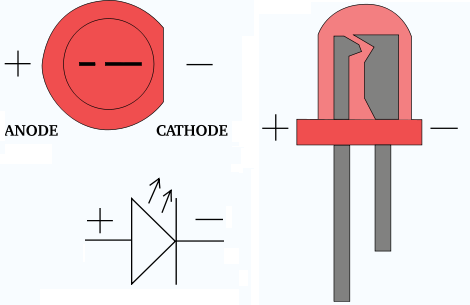
\includegraphics[width=5cm]{diagrammeLED.png}
  \end{center}
}

\begin{itemize}
	\item Why does the direct connection between the PSOC and the LED does not work well?
	Link that with the concept of maximum output current.
	\reponse{
        If we connect directly the LED on an output of the board, it switches on with a very low intensity. The board is simply unable to provide enough current for the LED.
	}
	\item Explain how the use of a \textit{buffer} circuit solves this problem.
	Draw the new block diagram of your system.
	\reponse{
		The use of a buffer allows to spread the command from the microcontroller while supplying more current to the LED.
	}
\end{itemize}
We will use a buffer circuit 74ACT244 whose specifications are given in the appendices.





\section{Use of the timer}
You are asked to make the LEDs blink at a given frequency. To do so, you will need a timer. 

This type of peripheral has a 8/16/24/32-bits register that is decremented at each clock cycle. When the value of this register reaches 0, the counter goes back to the specified period value and starts decrementing again. At the same time, a specific bit named TC rises (goes to '1') to warn of overflow (cf. datasheet of timer).
As a first step, you will write a program allowing to make the LED blink at a frequency of 1kHz.

\begin{itemize}
	\item Instantiate a Timer in the topDesign.cysch file. Set the period to cause on overflow at a frequency of 1kHz. What is the largest period of the timer? As a reminder, the highest clock rate available in a PSOC system is a BUS\_CLK at a rate of 24MHz.
	\reponse{If we want the LED to blink at a frequency of 1kHz, this corresponds to a period of 24000 instructions. The maximum period of this timer (on 16 bits) is $\frac{2^{16}-1}{24\cdot10^6} = 2731 \mu s $. }
	\item Add the launching of the timer in your program.
	\item In the main loop of your program:
	\begin{itemize}
		\item Check by polling if the timer has overflowed (ie. If the bit TC has risen to '1'). To do so, find the appropriate register that you need to poll. The datasheet mentions that the bit TC is ``sticky''. What does this mean? Do you need to reset the bit TC to zero after reading it or not? 
		\item Write a function that toggles LED4 (as well as one of the outputs on jumper J1 or J2) at the overflow frequency. This function must not be blocking: the high brightness LED must switch on at any time if the button is pressed.
	\end{itemize}
	\item Check the frequency with the oscilloscope.
	\item Modify the firmware (i.e. main.c) to obtain a period to 1s for the blinking of the LEDs. Since a 1s period cannot be achieved directly with a timer (see maximum period above), we rely on the firmware to count overflows of the timer until a 1s period is reached. 
\end{itemize}

\end{document}
